\documentclass[dvipsnames,10pt]{beamer}
\usepackage{ucltemplate}
\usepackage{tikz}
\usetikzlibrary{arrows,shapes, backgrounds, decorations.pathmorphing}
\usepackage{graphicx}
\usepackage{amssymb,amsmath}
\usepackage{listings}
\usepackage{multimedia}
\usepackage{algorithmic}
\usepackage{empheq}
\usepackage{makecell}
\usepackage[many]{tcolorbox}
\usepackage[labelformat=empty]{caption,subfig}

\setbeamertemplate{footline}[frame number]

\beamertemplatenavigationsymbolsempty

\setbeamertemplate{footline}[frame number]

\setbeamertemplate{navigation symbols}{}
\tikzstyle{na} = [baseline=-.5ex]

\tcbset{highlight math style={enhanced,
  colframe=red!60!black,colback=yellow!50!white,arc=4pt,boxrule=1pt,
  }}

\def\bx{\mathbf{x}}
\def\by{\mathbf{y}}

\renewcommand\theadalign{bc}
\renewcommand\theadfont{\bfseries}
\renewcommand\theadgape{\Gape[4pt]}
\renewcommand\cellgape{\Gape[4pt]}

\newcounter{sarrow}
\newcommand\xrsquigarrow[1]{%
\stepcounter{sarrow}%
\begin{tikzpicture}[decoration=snake]
\node (\thesarrow) {\strut#1};
\draw[->,decorate] (\thesarrow.south west) -- (\thesarrow.south east);
\end{tikzpicture}%
}

\title{Numerical aspects of relative Krein spectral shift function in acoustic scattering and Casimir energy computation}

\date{}

\begin{document}
\lstset{language=Python}
\tikzstyle{every picture}+=[remember picture]
%===============title page================
\begin{frame}

\vspace{1cm}

\titlepage
\vspace{-2cm}

\begin{center}
    $\text{Xiaoshu Sun}^{1}$
    \ $\text{Timo Betcke}^{1}$ \ $\text{Alexander Strohmaier}^{2}$\\
\vspace{0.5cm}
    ${}^{1}\text{University College London}$\\
    ${}^{2}\text{University of Leeds}$
\end{center}
\vspace{0.5cm}
\begin{center}
    ICOSAHOM 2020, 12th July
\end{center}
\end{frame}
%==================Intro: def and application===========
\begin{frame}
    \frametitle{Introduction: Definition and application}

    \vspace{.3cm}
    \begin{itemize}
        \item  \begin{minipage}{5cm}
    
    Sum of zero-point energy
        
        \begin{align*}
    \mathcal{E}(a) = \frac{1}{2}\sum_{n}\hbar\omega_{n}(a),
\end{align*}

    \end{minipage}
    \begin{minipage}{5cm}
        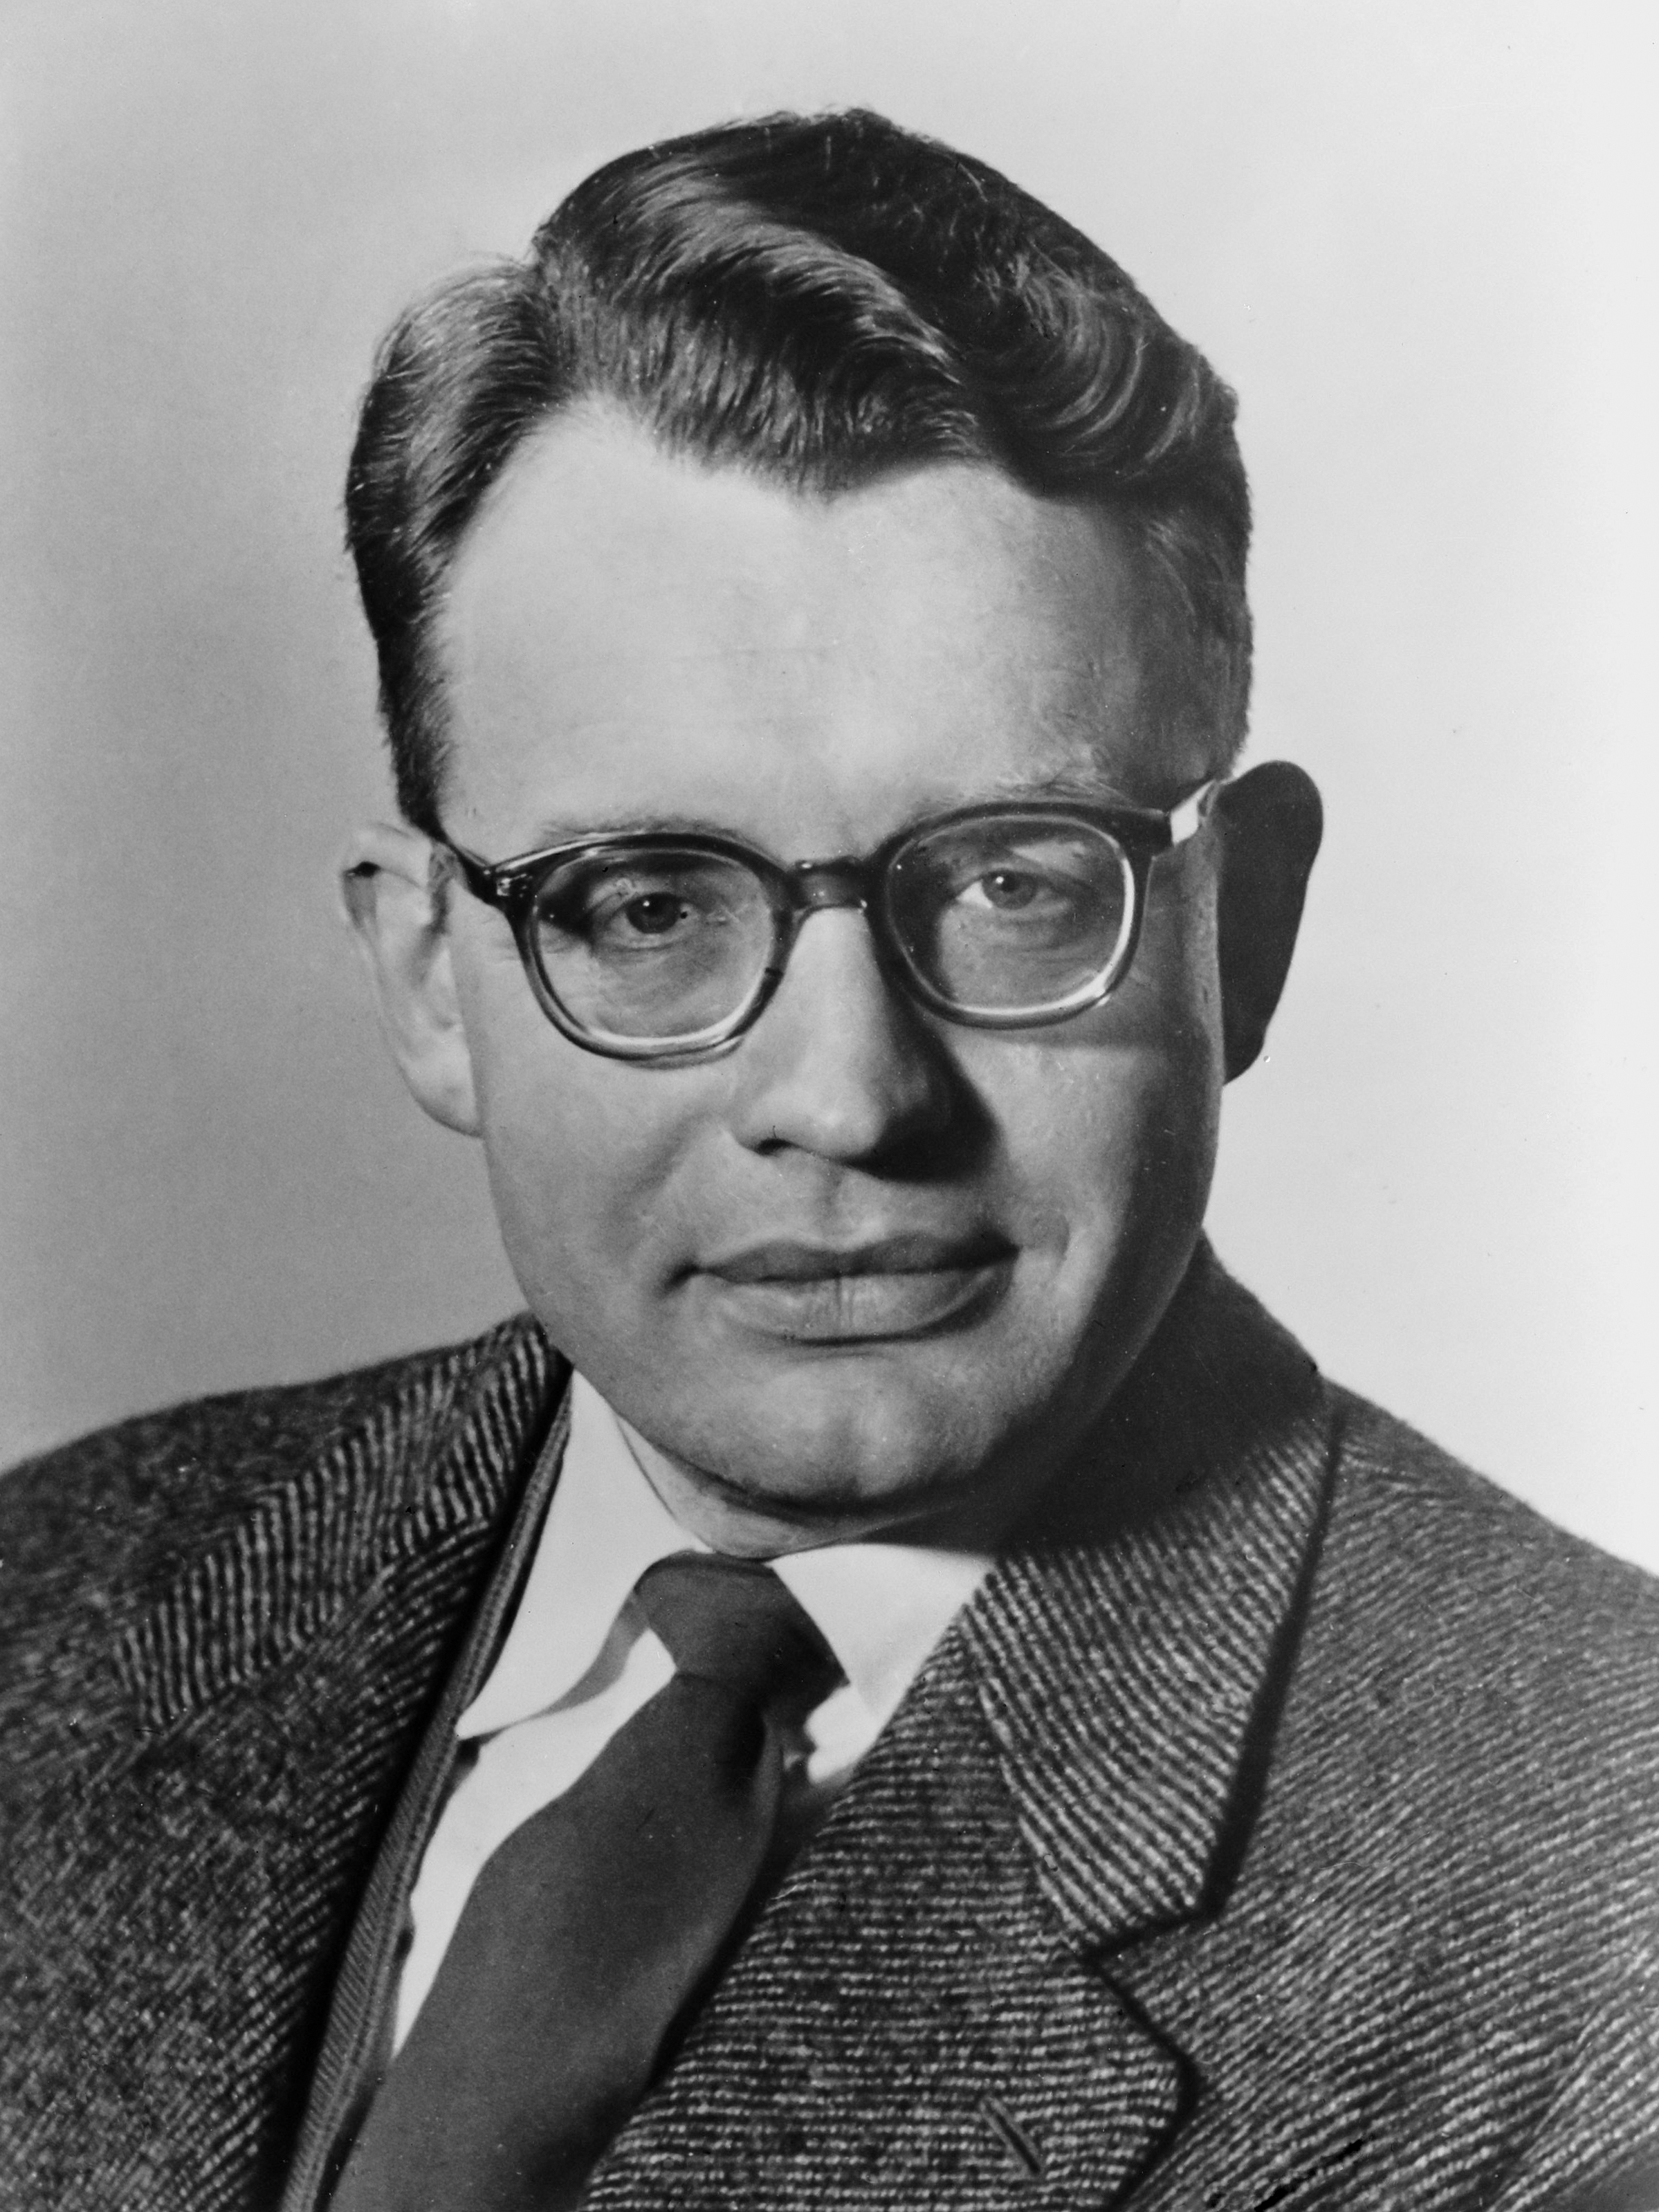
\includegraphics[width=2.4cm]{figs/Hendrik_Casimir_(1958).jpg}
        \hspace{0.05cm}
        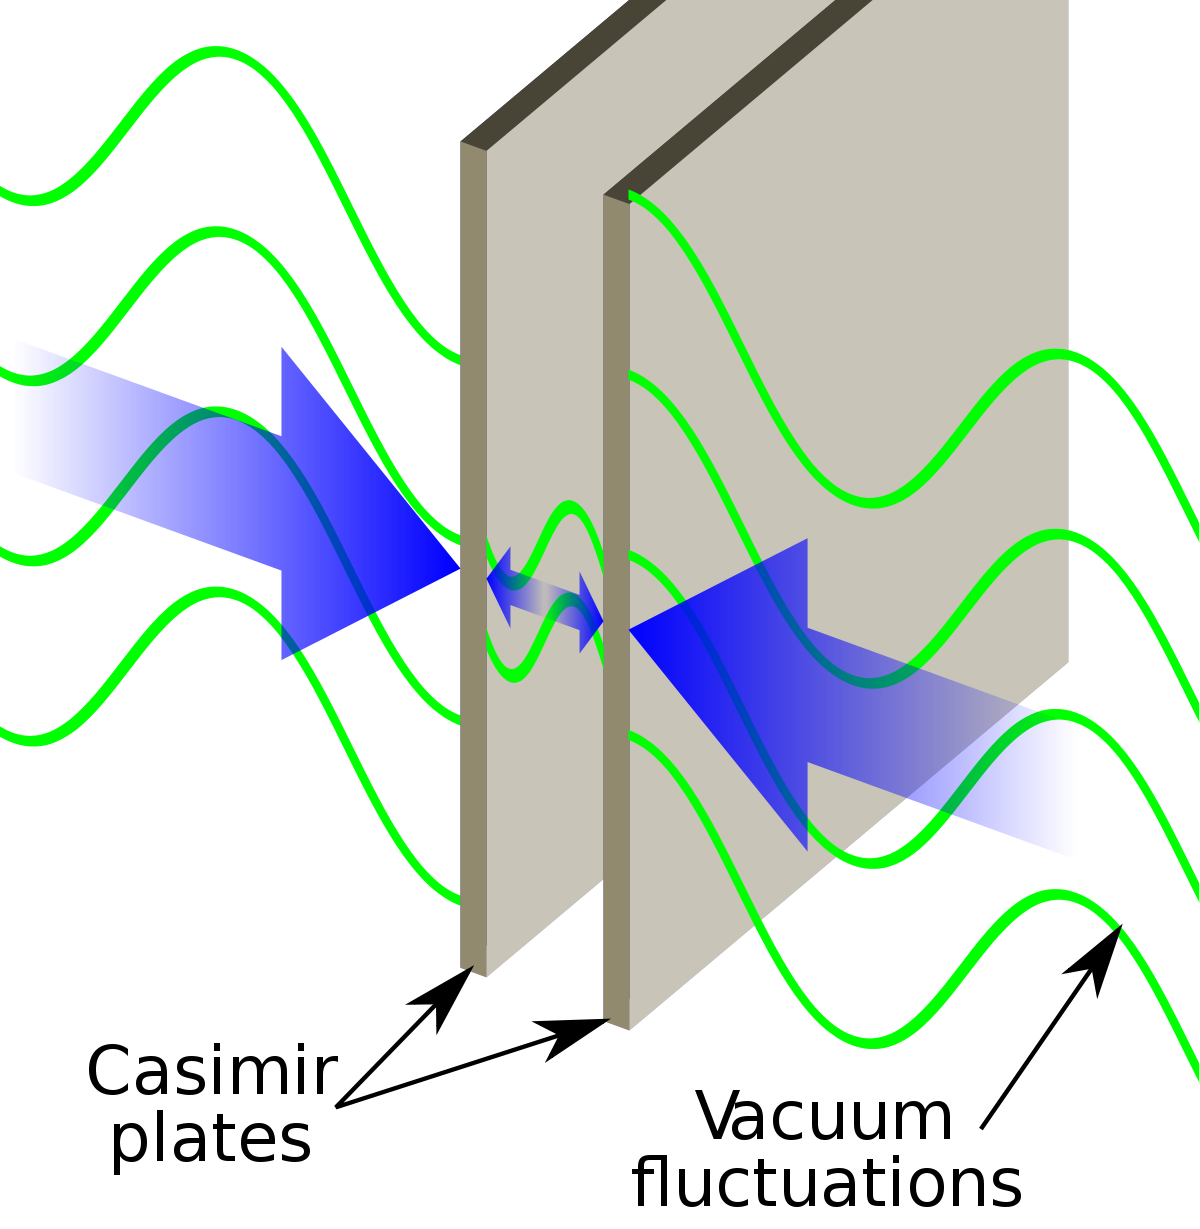
\includegraphics[width=2.4cm]{figs/Casimir_plates.png}
    \end{minipage}
    \vspace{0.3cm}
    \item \begin{minipage}{5cm}
    
    MEMS \\
    (Micro-Electro-Mechanical Systems)

    \end{minipage}
    \begin{minipage}{5cm}
    \centering
        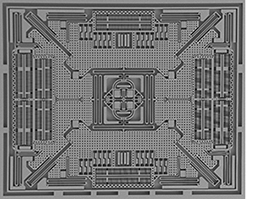
\includegraphics[width=3cm]{figs/MEMS.jpg}
    \end{minipage}
    \end{itemize}

\end{frame}
%==================Outline============================
\begin{frame}
    \frametitle{Outline}
\begin{itemize}
    \item Introduce the Krein spectral shift function (KSSF)
    \vspace{0.3cm}
    \item Derive the formula of Casimir energy via the KSSF
    \vspace{0.3cm}
    \item Speed up Casimir computations for large-scale practical problems
    \vspace{0.3cm}
    \item Numerical experiments 
\end{itemize}

\end{frame}
%================KSSF=================================
\begin{frame}
    \frametitle{Krein spectral shift function (KSSF)}
    \vspace{0.3cm}
    \begin{minipage}{5cm}
    
    \begin{align*}
    \xi(k) = \frac{1}{2\pi \mathrm{i}}\log\left(\frac{\det(S_{k})}{\det(S_{1,k})\cdots\det(S_{N,k})}\right)
\end{align*}
    \end{minipage}
    \begin{minipage}{2cm}
        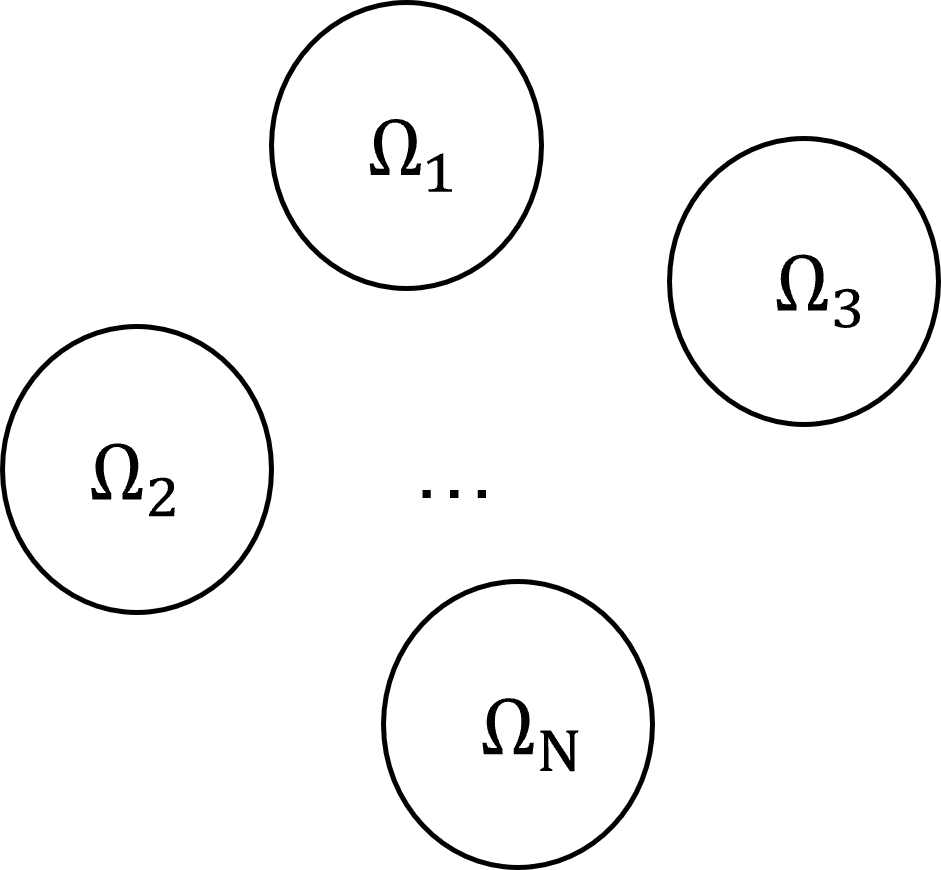
\includegraphics[scale = 0.5]{figs/Domain.png}
    \end{minipage}

\begin{itemize}
    \item $k$ is the wavenumber
    \item $S_{i,k} = I + 2T_{i,k}$ is the scattering matrix associated with the $i$th object
    \item $T_{i,k}$ is the $T$-matrix associated with the $i$th object
\end{itemize}
\begin{tcolorbox}
\textbf{Birman-Krein Formula}
    \begin{align*}
    \text{Tr}\left(f(\Delta^{\frac{1}{2}}) - f(\Delta_{0}^{\frac{1}{2}}) - \left(\sum_{j = 1}^{N}[f(\Delta_{j}^{\frac{1}{2}}) - f(\Delta_{0}^{\frac{1}{2}})]\right)\right)  = \int_{0}^{\infty}f'(k)\xi(k)dk
\end{align*}
\end{tcolorbox}

\end{frame}
%===============CasE from KSSF I======================
\begin{frame}
    \frametitle{Derive the Casimir energy via KSSF}
    \vspace{0.3cm}
    \begin{tcolorbox}
    \textbf{Birman-Krein Formula}
    \begin{align*}
    \text{Tr}\left(f(\Delta^{\frac{1}{2}}) - f(\Delta_{0}^{\frac{1}{2}}) - \left(\sum_{j = 1}^{N}[f(\Delta_{j}^{\frac{1}{2}}) - f(\Delta_{0}^{\frac{1}{2}})]\right)\right)  = \int_{0}^{\infty}f'(k)\xi(k)dk
\end{align*}
\end{tcolorbox}
When $f(x) = x$:
\begin{align*}
        \emph{\text{Tr}}\left(\Delta^{\frac{1}{2}} + (N - 1)\Delta_{0}^{\frac{1}{2}} - \sum_{i = 1}^{N}\Delta_{j}^{\frac{1}{2}}\right)  = 
        \int_{0}^{\infty}\xi(k)dk
    \end{align*}
\begin{tcolorbox}
    \textbf{Casimir energy formula\footnote{Hanisch F, Strohmaier A, Waters A. A relative trace formula for obstacle scattering[J]. arXiv preprint arXiv:2002.07291, 2020.} ---
    Scattering matrix method}
    
    $$\mathcal{E}_{\textbf{sca}} = \frac{\hbar c}{2}\int_{0}^{\infty}\xi(k)dk$$
\end{tcolorbox}
\end{frame}
%==============CasE from KSSF II=================
\begin{frame}
    \frametitle{Derive the Casimir energy via KSSF}
    \vspace{0.3cm}
    \begin{itemize}
        \item $\Omega$: a domain assembling from individual objects $\Omega_{i}$
        \item $V_{k}$: the single-layer boundary operator defined on the boundary 
    $\partial\Omega = \bigcup_{i = 1}^{N}\partial\Omega_{i}$
    \item $\tilde{V}_{k}$: the ``diagonal part'' of $V_{k}$ by restricting the integral 
    kernel to the subset $\bigcup_{i = 1}^{N}\partial\Omega_{i}\times\partial\Omega_{i}\subset\partial\Omega\times\partial\Omega$ 
    \end{itemize}
    \begin{minipage}{5cm}
    Define:
    \begin{align*}
        \Xi(k) = \log\det\left(V_{k}\tilde{V}_{k}^{-1}\right)
    \end{align*}
    \end{minipage}
    \begin{minipage}{2cm}
        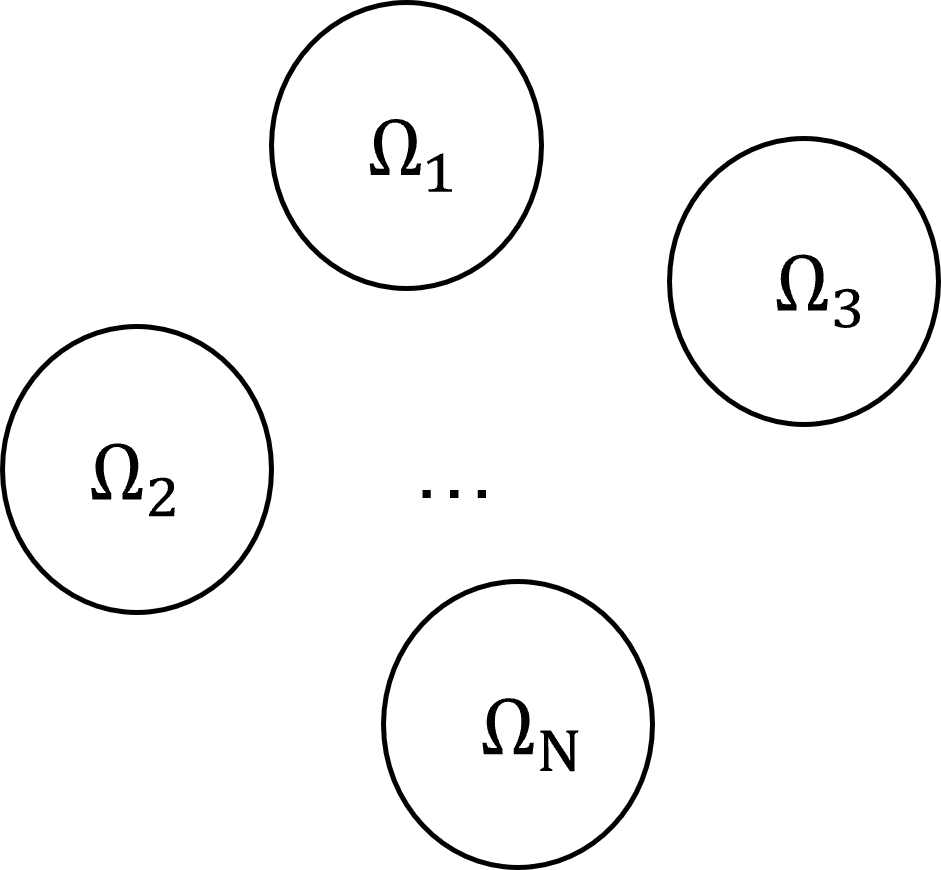
\includegraphics[scale = 0.5]{figs/Domain.png}
    \end{minipage}
    \begin{tcolorbox}
    \textbf{Relation between the single-layer operator and KSSF}
    
        For $k>0$,
        \begin{align*}
        -\frac{1}{\pi}\text{Im}\Xi(k) = \frac{\mathrm{i}}{2\pi}(\Xi(k) - \Xi(-k)) = \xi(k)
    \end{align*}
    \end{tcolorbox}
\end{frame}
%==============CasE from KSSF III=================
\begin{frame}
    \frametitle{Derive the Casimir energy via KSSF}
      \begin{tcolorbox}
    \textbf{Relation between the single-layer operator and KSSF}
    
        For $k>0$,
        \begin{align*}
        -\frac{1}{\pi}\text{Im}\Xi(k) = \frac{\mathrm{i}}{2\pi}(\Xi(k) - \Xi(-k)) = \xi(k)
    \end{align*}
    \end{tcolorbox}
    This relation can help to derive:
    \begin{tcolorbox}
    \textbf{Casimir energy formula\footnote{Hanisch F, Strohmaier A, Waters A. A relative trace formula for obstacle scattering[J]. arXiv preprint arXiv:2002.07291, 2020.} ---
    Single-layer operator method}
    
    $$\mathcal{E}_{\textbf{slp}} =  -\frac{\hbar c}{2\pi}\int_{0}^{\infty}\Xi(\mathrm{i}k)dk$$
\end{tcolorbox}
\end{frame}
%=============Compute CasE====================
\begin{frame}
    \frametitle{Compute the Casimir energy}
    \begin{tcolorbox}
\textbf{Casimir energy formula ---
    Single-layer operator method}
    
    $$\mathcal{E}_{\textbf{slp}} =  -\frac{\hbar c}{2\pi}\int_{0}^{\infty}\Xi(\mathrm{i}k)dk = -\frac{\hbar c}{2\pi}\int_{0}^{\infty}\log\det\left(V_{\mathrm{i}k}\tilde{V}_{\mathrm{i}k}^{-1}\right)dk$$
\end{tcolorbox}

\begin{itemize}
    \item Task 1: Compute the integrand $\log\det\left(V_{\mathrm{i}k}\tilde{V}_{\mathrm{i}k}^{-1}\right)$ by using the Galerkin discretization form of operators
    \vspace{0.3cm}
    \item Task 2: Evaluate the integral $\int_{0}^{\infty}\log\det\left(V_{\mathrm{i}k}\tilde{V}_{\mathrm{i}k}^{-1}\right)dk$ via the trapezoidal rule
\end{itemize}


\end{frame}
%============Compute CasE Basis functions=================
\begin{frame}
    \frametitle{Compute the Casimir energy}
    \vspace{0.3cm}
\textbf{Task 1}: Compute the integrand $\log\det\left(V_{\mathrm{i}k}\tilde{V}_{\mathrm{i}k}^{-1}\right)$ by using the Galerkin discretization form of operators
\vspace{0.2cm}

\textbf{Single-layer boundary operator:}
\begin{align*}
    (V_{k}\mu)(\boldsymbol{x}) := \int_{\Gamma}g_{k}(\boldsymbol{x},\boldsymbol{y})\psi(\boldsymbol{y})dS_{\boldsymbol{y}}, \ \ \ \ \ 
    \text{for}\ \mu\in H^{-\frac{1}{2}}(\Gamma) \  \text{and} \ \boldsymbol{x}\in\Gamma,
\end{align*}
where \begin{align*}
    g_{k}(\boldsymbol{x},\boldsymbol{y}) = \begin{cases}
          \frac{\mathrm{i}}{4}H_{0}^{(1)}(k|\boldsymbol{x}-\boldsymbol{y}|), \ \ \ \ &\text{for} \ d = 2\\
          \frac{e^{ik|\boldsymbol{x}-\boldsymbol{y}|}}{4\pi|\boldsymbol{x} - \boldsymbol{y}|}, \ \ \ \ &\text{for} \ d = 3.
        \end{cases}
\end{align*}
\vspace{0.2cm}

To discretize it, we define the continuous piecewise linear basis functions:
\begin{align*}
    P_{h}^{1}(\Gamma) := \text{span}\{\phi_{j}\} \subset H^{-\frac{1}{2}}(\Gamma)
\end{align*}
with 
\begin{align*}
    \phi_{j}(\boldsymbol{x}_{j}) = \begin{cases}
        1, & i = j,\\
        0, & i\neq j.
    \end{cases}
\end{align*}

\end{frame}
%===========Compute CasE Galkerkin form==============
\begin{frame}
    \frametitle{Compute the Casimir energy}
    \textbf{Task 1}: Compute the integrand $\log\det\left(V_{\mathrm{i}k}\tilde{V}_{\mathrm{i}k}^{-1}\right)$ by using the Galerkin discretization form of operators
\vspace{0.3cm}

\textbf{Matrix representation of Galerkin discretised single-layer boundary operator:}

\begin{align*}
    \mathsf{V}_{k} = \begin{bmatrix}
        \mathsf{V}_{11}(k) & \cdots & \mathsf{V}_{1N}(k) \\
        \vdots & \ddots & \vdots \\
        \mathsf{V}_{N1}(k)  & \cdots & \mathsf{V}_{NN}(k) \\
\end{bmatrix}, \ 
\tilde{\mathsf{V}}_{k} =  \begin{bmatrix}
        \mathsf{V}_{11}(k)     & \cdots & 0 \\
    \vdots & \ddots & \vdots \\
    0          & \cdots & \mathsf{V}_{NN}(k) \\
\end{bmatrix},
\end{align*}
where \begin{align*}
    \mathsf{V}_{ij}^{(m,n)} (k) = \langle V_{ij}(k)\phi_{m}^{(i)}, \phi_{n}^{(j)}\rangle = 
    \int_{\Gamma}\overline{\phi_{n}^{(j)}}(\boldsymbol{x})\int_{\Gamma}g_{k}(\boldsymbol{x}, \boldsymbol{y})\phi_{m}^{(i)}(\boldsymbol{y})dS_{\boldsymbol{y}}dS_{\boldsymbol{x}}
\end{align*}   
and $\boldsymbol{\phi}^{(i)} = \begin{bmatrix}
    \phi_{1}^{(i)} & \phi_{2}^{(i)} & \dots & \phi_{N}^{(i)}
\end{bmatrix}\subset P_{h}^{1}(\Gamma)$  is the set of basis functions defined on the $i$th object.
\end{frame}
%===========Compute CasE trapezoidal rule============
\begin{frame}
    \frametitle{Compute the Casimir energy}
    \textbf{Task 2}: Evaluate the integral $\int_{0}^{\infty}\log\det\left(V_{\mathrm{i}k}\tilde{V}_{\mathrm{i}k}^{-1}\right)dk$ via the trapezoidal rule
    
    \begin{itemize}
        \item (Left) The integrand value $\log\det\left(V_{\mathrm{i}k}\tilde{V}_{\mathrm{i}k}^{-1}\right)$ exponentially decay with the increasing $k$.
        \item (Right) By changing the variable from $k$ to $k = -\log(y)$, we can apply the normal trapezoidal rule to compute the integral.
    \end{itemize}
    
\begin{figure}[H]
    \begin{minipage}[b]{.47\textwidth}
    \centering
    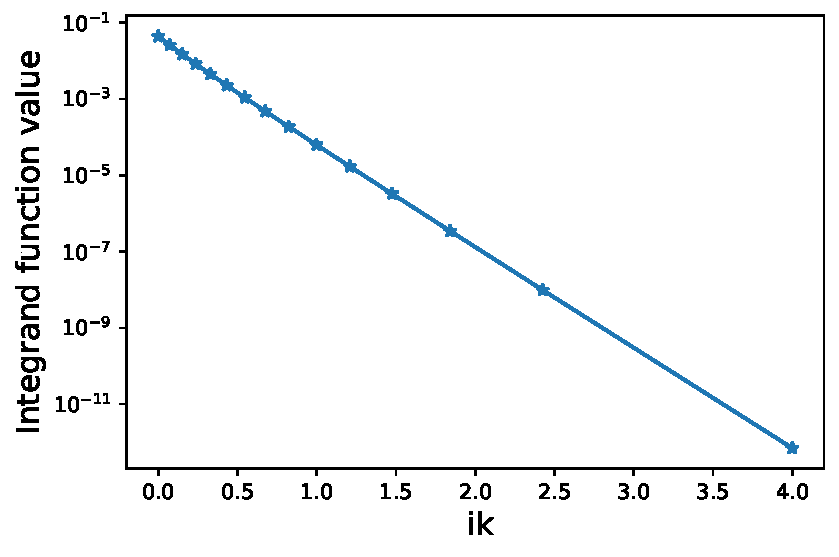
\includegraphics[width=1\textwidth]{figs/integ_exp_decay.pdf}
    \end{minipage}
    \hfill
    \begin{minipage}[b]{.47\textwidth}
    \centering
    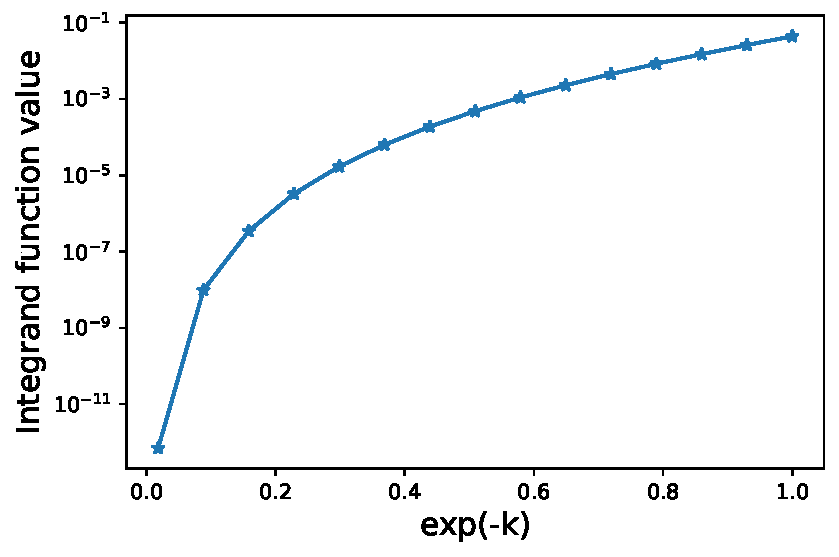
\includegraphics[width=1\textwidth]{figs/integ_exp_not_decay.pdf}
    \end{minipage}
    \end{figure}


\end{frame}
%========= inverse free========
\begin{frame}
    \frametitle{Inverse-free methods for large-scale problems}
Most of the eigenvalues of $V_{\mathrm{i}k}\tilde{V}_{\mathrm{i}k}^{-1}$ are around 1, which contribute nothing on the log determinant.

\begin{figure}[H]
    \centering
    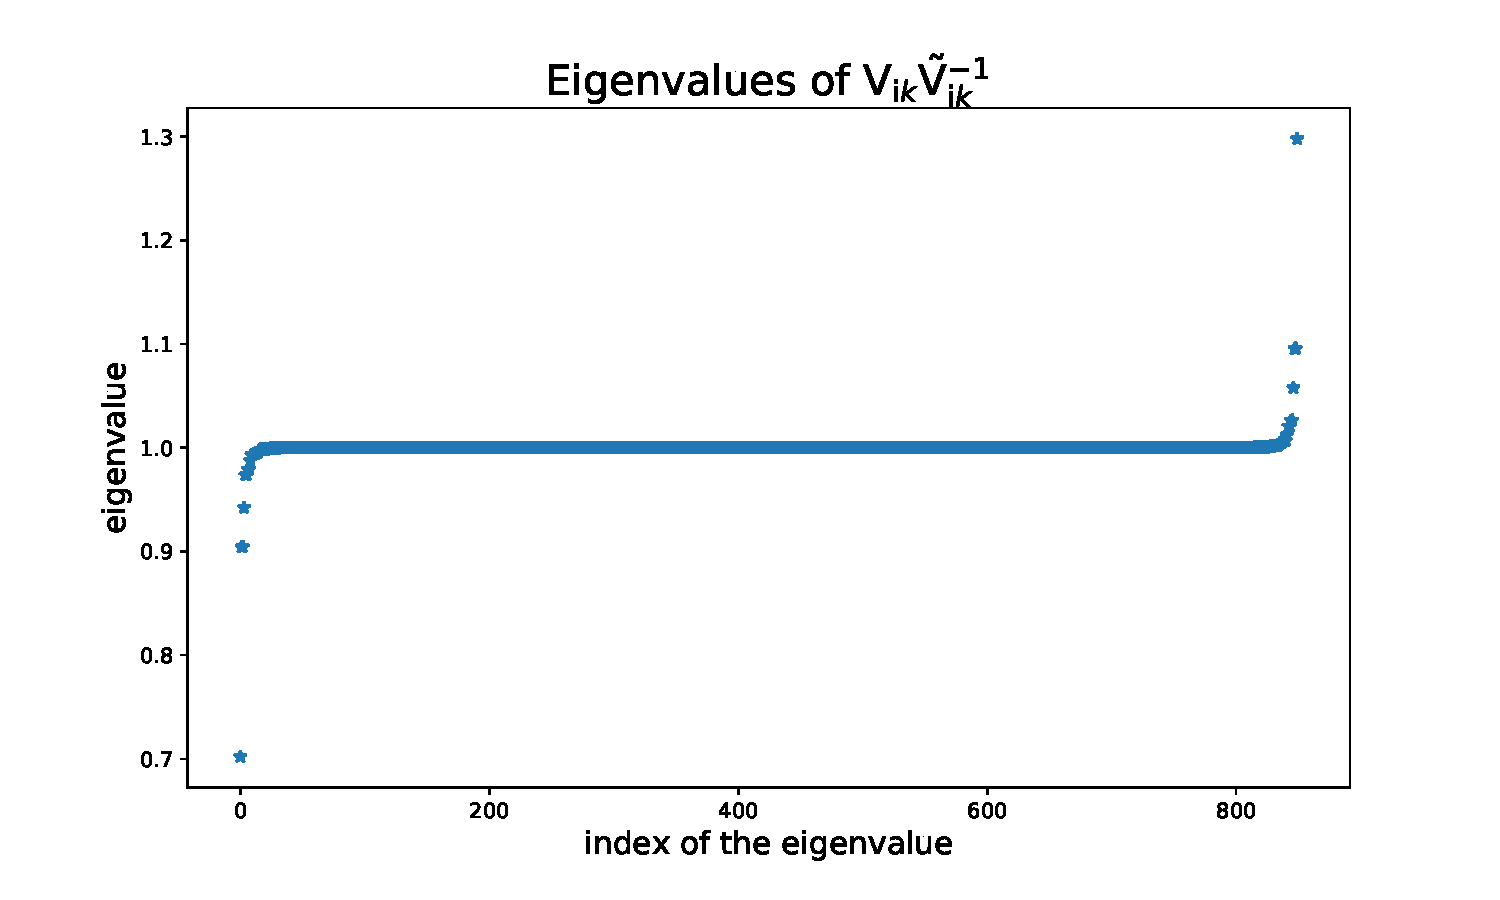
\includegraphics[scale = 0.35]{figs/eigenvalue_of_VVtilde.pdf}
    \caption{The eigenvalues of the matrix $\mathsf{V}_{\mathrm{i}k}\tilde{\mathsf{V}}_{\mathrm{i}k}^{-1}$ when $\mathrm{i}k = 0.8\mathrm{i}$.}

\end{figure}
\end{frame}
%===========inverse free I========
\begin{frame}
    \frametitle{Inverse-free methods for large-scale problems}
    \vspace{0.3cm}
\textbf{Method I:} Inverse-free Krylov subspace method for computing $p$ smallest (or largest) eigenvalues of  $\mathsf{V}_{\mathrm{i}k}\tilde{\boldsymbol{x}} = \lambda \tilde{\mathsf{V}}_{\mathrm{i}k}\tilde{\boldsymbol{x}}$.
\begin{tcolorbox}
    \begin{algorithm}
    \SetAlgoLined
    Input: Symmetric  $A\in\mathbb{R}^{n\times n}$, s.p.d  $B\in\mathbb{R}^{n\times n}$ and
    $X^{(1)} \in\mathbb{R}^{n\times p}$ with $X^{(1)*}BX = I_{p}$ and $m\geq 1$\\
    Output: The approximated $p$ smallest eigenvalues of $A\boldsymbol{x} = \lambda B\boldsymbol{x}$\\
    \begin{algorithmic}[1]
        \STATE Set $\Theta^{(1)} = \text{diag}(X^{(1)*}AX^{(1)})$
        \FOR {$k = 1, 2, \dots$} 
                \FOR {$i = 1, 2, \dots, p$}
                    \STATE Construct a basis $\hat{Z_{i}}$ of the $i$th Krylov subspace $K_{m}(A - \theta_{i}^{(k)}B, x_{i}^{(k)})$ with dimension $m$
                    \STATE Orthonormalize $\left[\hat{Z_{1}} \cdots \hat{Z_{p}}\right]$ to obtain $Z$
                    \STATE Project $A$ and $B$ on $Z$: $A_{m} = Z^{*}AZ$, $B_{m} = Z^{*}BZ$
                    \STATE Compute $p$ smallest eigenpairs $(\theta_{i}, u_{i})$, $1\leq i \leq p$ of the matrix pencil $(A_{m}, B_{m})$
                    \STATE $\Theta^{(k+1)} = \text{diag}(\theta_{1}, \dots, \theta_{p})$; $X^{(k+1)} = ZU$, $U = (u_{1} \cdots u_{p})$
                \ENDFOR
        \ENDFOR
        \end{algorithmic}
    \caption{Inverse-free Krylov subspace method for computing $p$ smallest eigenvalues of the generalized eigenvalue problem $A\boldsymbol{x} = \lambda B\boldsymbol{x}$}
    \label{Alg for computing the evals}
    \end{algorithm}
\end{tcolorbox}

\end{frame}
%===========inverse free II========
\begin{frame}
    \frametitle{Inverse-free methods for large-scale problems}
    \vspace{0.3cm}
\textbf{Method II:} LU decomposition for inverting the matrix.
\begin{align*}
    \tilde{\mathsf{V}}_{\mathrm{i}k}^{-1}
=  \begin{bmatrix}
    \mathsf{V}_{11}^{-1}(\mathrm{i}k)    & \cdots & 0 \\
    \vdots                              & \ddots & \vdots \\
       0       & \cdots        & \mathsf{V}_{NN}^{-1} (\mathrm{i}k)\\
\end{bmatrix}
\end{align*}
 For each block $\mathsf{V}_{ii} = \mathsf{V}_{ii}(\mathrm{i}k)$, for $i = 1, 2, \dots, N$:
 \begin{itemize}
     \item Compute its LU decomposition $\mathsf{V}_{ii} = \mathsf{L}_{ii}\mathsf{U}_{ii}$
     \item Solve the linear system $\mathsf{L}_{ii}\mathsf{U}_{ii}\boldsymbol{x_{j}} = \boldsymbol{e}_{j}$, for $j = 1, 2, \dots, N_{\mathsf{V}_{ii}}$
     \item $\mathsf{V}_{ii}^{-1} = \begin{bmatrix}
    \boldsymbol{x}_{1} & \cdots & \boldsymbol{x}_{N_{\mathsf{V}_{ii}}}
\end{bmatrix}$
 \end{itemize}
\end{frame}
%===========inverse free II========
\begin{frame}
    \frametitle{Inverse-free methods for large-scale problems}
\textbf{Method II:} LU decomposition for inverting the matrix.
    \vspace{0.3cm}

\begin{itemize}
    \item Define the inverse of the matrix $\tilde{\mathsf{V}}_{\mathrm{i}k}$ computed by the inverse-free $LU$ decomposition method as 
$\tilde{\mathsf{V}}_{\mathrm{i}k}^{-1,\text{LU}}$.
\vspace{0.2cm}
\item Compute the basis of the Krylov subspace 
$K_{m}(\mathsf{V}_{\mathrm{i}k}\tilde{\mathsf{V}}_{\mathrm{i}k}^{-1,\text{LU}}, \boldsymbol{b})$ and project
via the Arnoldi iterations and project $\mathsf{V}_{\mathrm{i}k}\tilde{\mathsf{V}}_{\mathrm{i}k}^{-1,\text{LU}}$ onto it to obtain the Hessenberg matrix $H_{m}$.
\vspace{0.2cm}

\item The eigenvalues of Hessenberg matrix can be used to approximate extreme eigenvalues of $\mathsf{V}_{\mathrm{i}k}\tilde{\mathsf{V}}_{\mathrm{i}k}^{-1,\text{LU}}$

\end{itemize}
\end{frame}
%===========Compare two inverse free methods=
\begin{frame}
    \frametitle{Compare two inverse-free methods}
\begin{figure}[H]
    \centering
    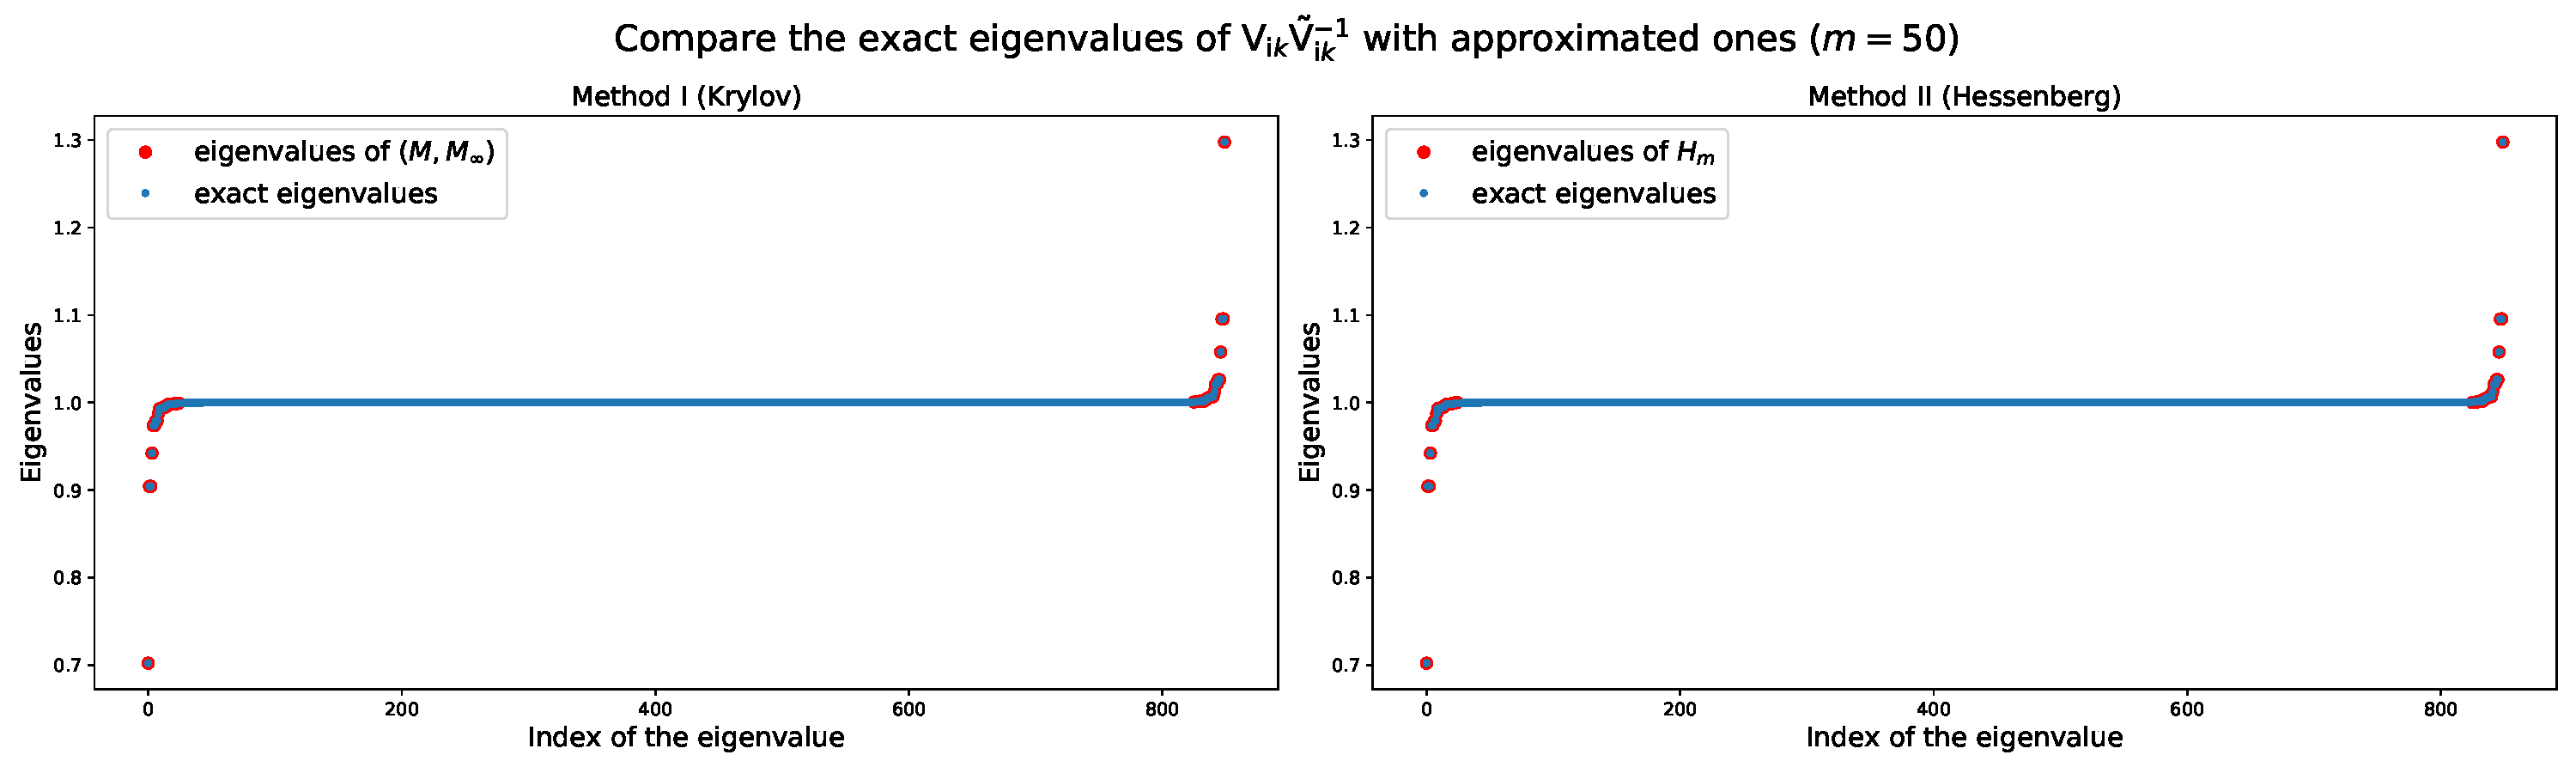
\includegraphics[scale = 0.23]{figs/Method_GEP_m_50.pdf}
\end{figure}
\begin{figure}[H]
    \centering
    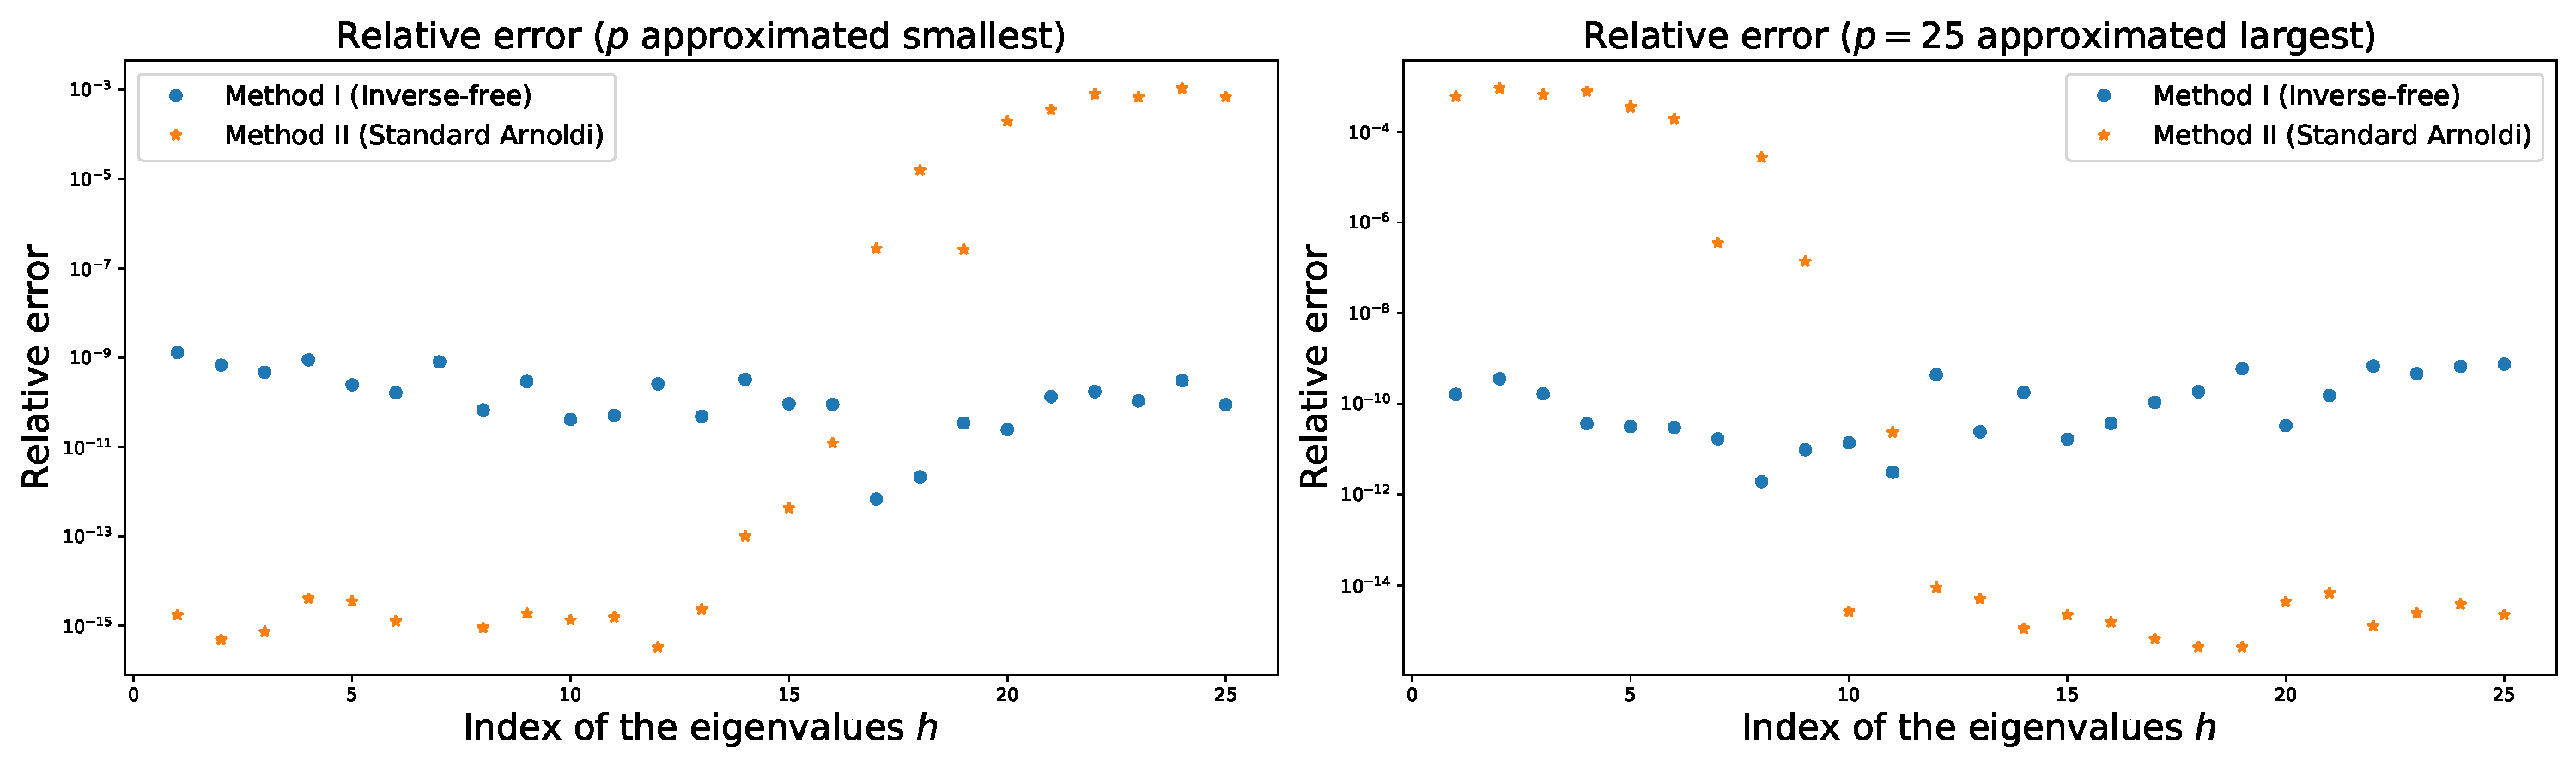
\includegraphics[scale = 0.23]{figs/rel_err_m_50.pdf}
\end{figure}
\end{frame}
%===========Compare two inverse free methods=
\begin{frame}
    \frametitle{Compare two inverse-free methods}
\begin{figure}[H]
    \centering
    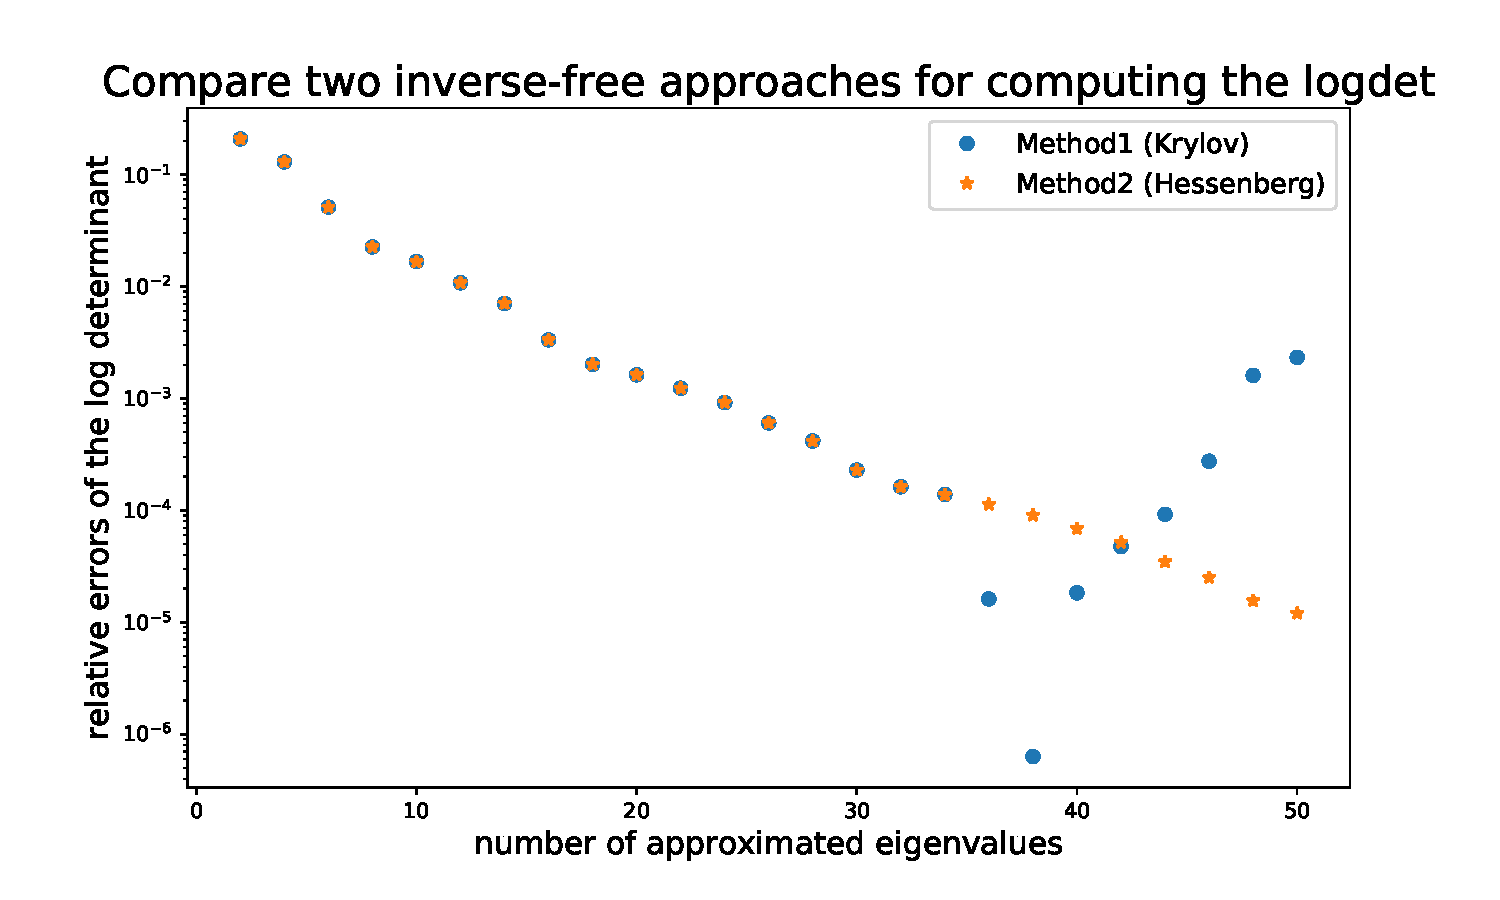
\includegraphics[scale = 0.45]{figs/compare_two_inv_free_approaches.pdf}
\end{figure}
\end{frame}
\begin{frame}{Summary}
\begin{itemize}
    \item Casimir energy can be computed via evaluating the log determinant of the single-layer boundary operators
    
    \item Efficiently computing the Casimir enengy by avoiding computing any inverse matrix and only approximating multiple extreme eigenvalues.
    
    \item Next step is to focus on the maxwell case, which needs us to change the operator to the electric field boundary operator. 
\end{itemize}
\end{frame}
\begin{frame}{Papers}

    \begin{itemize}
        \item Hanisch F, Strohmaier A, Waters A.\textit{ A relative trace formula for obstacle scattering}. arXiv preprint arXiv:2002.07291, 2020. 
        \textbf{[KSSF and Casimir energy]}
        
        \item Quillen P, Ye Q. \textit{A block inverse-free preconditioned Krylov subspace method for symmetric generalized eigenvalue problems}. Journal of computational and applied mathematics, 2010, 233(5): 1298-1313.
        \textbf{[Inverse-free Krylov subspace method for generalized eigenvalue problem]}
        
        \item  Saad Y. \textit{Numerical methods for large eigenvalue problems: revised edition}. Society for Industrial and Applied Mathematics, 2011.
        \textbf{[Arnoldi iteration]}
    \end{itemize}

\end{frame}
\end{document}

